% \'Equations différentielles et systèmes dynamiques en temps continu. Existence, unicité des solutions. Recherche des équilibres et linéarisation. Classification des équilibres en dimensions 1 et 2.

%-------------------------------------------------------------------------------
\paragraph*{Objectif.} 
On s'intéresse à une fonction 
$$
\begin{array}{rrcl}
  y : & \Rbb & \mapsto & \Rbb^n \\
  & t & \rightarrow & y(t) = [y_1(t) \dots y_n(t)]^\top 
\end{array}
$$
qui soit solution d'une équation {\em fonctionnelle} de la forme
$$
\nabla y(t) = F(y(t))
$$
où $F$ est une fonction de $\Rbb^n$ dans $\Rbb^n$. Une telle équation est appelée {\em équation différentielle ordinaire} (EDO, alias {\em ODE} en anglais).

Comme la notation le laisse entendre, la variable $t$ décrit typiquement un temps et $y(t)$ l'évolution d'un système à $n$ coordonnées au cours du temps partialant d'une {\em condition initiale}
$$
y(t_0) = y_0.
$$
En notant $\dot y$ la dérivée de $y$ par rapport au temps, un tel {\em système dynamique} s'écrit donc
$$
\left\{\begin{array}{rcl}
        y(t_0) & = & y_0, \\
        \dot y & = & F(y).
       \end{array}\right.
$$

%-------------------------------------------------------------------------------
\paragraph*{Deux modèles classiques.}
\begin{description}
 \item[Lotka-Volterra:] $y(t) = [N(t) \; P(t)]^\top$ avec $N(t) =$ nombre de proies au temps $t$, $(t) = $ nombre prédateurs au temps $t$:
 $$
 \left\{ \begin{array}{rcl} 
  \dot N & = & r N - c N P \\
  \dot P & = & b N P  - m P
 \end{array} \right.
 $$
 \item[SIR :] $y(t) = [S(t) \; I(t) \; R(t)]^\top$ avec $S(t) =$ nombre de susceptibles au temps $t$ ,$I(t) =$ nombre d'infectés et $R(t) =$ nombre de 'remis' ({\em recovered}) :
 $$
 \left\{ \begin{array}{rcl} 
  \dot S & = & - r S I \\
  \dot I & = & r S I - a I \\
  \dot R & = & a I \\
 \end{array} \right.
 $$
 (modèle à compartiments).
\end{description}

Ces deux modèles sont fondés sur des sytèmes d'équations différentielles en dimension plus grande que 1 et non linéaires.

%-------------------------------------------------------------------------------
%-------------------------------------------------------------------------------
\section{Exemple en 1D et solution maximale, stabilité} \label{sec:EquaDiff-1DsolMaximale}
%-------------------------------------------------------------------------------

%-------------------------------------------------------------------------------
\paragraph*{ODE linéaire en dimension 1 : modèle de Malthus.}
L'EDO la plus simple en dimension 1 est l'équation linéaire
$$
\dot y = r y
$$
dont la solution est connue : 
$$
y(t) = a_0 e^{rt}.
$$
Le paramètre $a_0$ est alors déterminé par une condition 'initiale' : en imposant que $y(t_0) = y_0$, il vient
$$
a_0 = y_0 e^{-t_0} 
\qquad \Rightarrow \qquad
y(t) = y_0 e^{r(t-t_0)}.
$$
Ce modèle est connu en dynamique des population sous le nom de {\em modèle de Malthus} : il suppose que l'accroissement de la population est directement proportionnel à sa taille. Ce modèle n'inclue pas de limitation de la taille de la population et en prévoit donc une croissance indéfini (pour $r > 0$).


%-------------------------------------------------------------------------------
\subsection{Solution maximale} 
%-------------------------------------------------------------------------------

\begin{definition*}[Solution du problème de Cauchy]
  Soit $F : \Rbb^n \mapsto \Rbb^n$, $I$ un ouvert de $\Rbb$, $t_0 \in I$ et $y_0 \in \Rbb$. La fonction $f : I \mapsto \Rbb^n$ est dite solution du \emph{problème de Cauchy}, 
  $$
  \left\{\begin{array}{rcl}
          y(t_0) & = & y_0, \\
          \dot y & = & F(y).
        \end{array}\right.
  $$
  sur $I$ si $f(t_0) = y_0$ et $\forall t \in I: \dot f(t) = F(f(t))$.
\end{definition*}

\begin{theorem*}[Cauchy-Lipschitz]
  Si $F$ est est $C^1$ par morceaux, il existe une unique solution $f$ sur $I$ au problème de Cauchy qui soit maximale au sens où si $g$ est également solution sur $J$, alors $J \subset I$ et $g(t) = f(t)$ pour tout $t \in J$. $f$ est appelée solution maximale et $I$ intervalle maximal.
\end{theorem*}

\remark
$f(t) = y_0 e^{r(t-t_0)}$ est donc l'unique solution du problème $\{y_0 = y(t_0), \; \dot y = r y\}$ sur l'intervalle maximal $\Rbb$.

%-------------------------------------------------------------------------------
\begin{exercise*}
  Déterminer la solution et l'intervalle maximal du problème
  $$
  \{y(0) = 1, \; \dot y = -c y^2\}.
  $$
\end{exercise*}

\solution{
  On remarque que
  \begin{align*}
    \dot y & = -c y^2 & 
    & \Leftrightarrow & 
    c & = - \frac{\dot y}{y^2} = \frac{\partial}{\partial t} \frac1y \\
    \text{donc} \qquad 
    \frac1y & = a + ct & 
    & \Leftrightarrow &
    y(t) & = \frac1{a + ct} \qquad \text{pour } t \neq -\frac{a}c.
  \end{align*}
  La condition $y(0) = 1$ impose alors que $a = 1$. $f(t) = (1+ ct)^{-1}$ est donc solution maximale sur l'intervalle (maximal) $\Rbb \setminus \{-1/c\}$.
}

%-------------------------------------------------------------------------------
\subsection{Point d'équilibre, stabilité} 
%-------------------------------------------------------------------------------

\begin{definition*}[Point d'équilibre]
  $x^* \ \Rbb^n$ est un point d'équilibre de l'ODE $\dot y = F(y)$ si $F(x^*) = 0$.
\end{definition*}

\begin{definition*}[Stabilité ($n = 1$)]
  Pour $n = 1$, un équilibre $x^*$ est dit (asymptotiquement) stable si il existe $\varepsilon > 0$ tel que pour tout $y_0 \in (x^* - \varepsilon, x^* + \varepsilon)$, la condition initiale $y(0) = y_0$ implique que 
  $$
  \lim_{t \rightarrow \infty} y(t) = x^*.
  $$
  Dans le cas contraire, il est dit {\em instable}. Le caractère stable ou instable d'un équilibre définit sa {\em nature}.
\end{definition*}

\remark
Un équilibre est donc stable si toute (petite) perturbation $\varepsilon$ autour de $x^*$ laisse le système retourner dans l'état $x^*$.


%-------------------------------------------------------------------------------
\paragraph*{Modèle de Verhulst.}
Une façon simple d'empêcher la croissance indéfinie de la population prédite par le modèle de Malthus consiste à supposer que le taux de reproduction $\dot y / y$ décroît linéairement avec la taille de la population : 
$$
\dot y / y = r - cy
\qquad \Leftrightarrow \qquad
\dot y = y(r - cy) = ry - c y^2.
$$
Ce modèle est connu sous le nom de {\em modèle de Verhulst}. On suppose typiquement que les paramètres $r$ et $c$ sont positifs.
\begin{description}
  \item[Points d'équilibre:] $x^* = 0$ et $x^* = K := r/c$ sont des points d'équilibre car alors $\dot y = F(x^*) = 0$.
  \item[Solution pour $y_0 \in \{0, K\}$:] la fonction $y(t)$ reste constante (car $\dot y(t) \equiv 0$).
  \item[Solution pour $0 < y_0 < K$:]
  On obtient une solution de cette équation en remarquant que, pour $t$ tel que $0 < y(t) < K$, on a
  $$
  r 
  = \frac{r \dot y}{y(r - cy)}
  = \frac{\dot y}{y} + \frac{c \dot y}{r - cy}
  = \frac{\partial}{\partial t} \left(\log y - \log (r - cy) \right)
  = \frac{\partial}{\partial t} \left(\log \left(\frac{y}{r - cy}\right)\right).
  $$
  En supposant que $0 < y < K$, on obtient comme solution 
  \begin{align*}
    \log \left(\frac{y}{r - cy}\right) & = rt + \log b
    \qquad \Leftrightarrow \qquad 
    \frac{y}{r - cy} = b e^{rt}
    \qquad \Leftrightarrow \qquad
    y(1 + c b e^{rt}) = r b e^{rt} \\
    \Leftrightarrow \qquad 
    y = \frac{rb e^{rt}}{1 + cb e^{rt}} & = \frac{K a_0 e^{rt}}{1 + a_0 e^{rt}}
    \qquad \text{avec } a_0 = cb.
  \end{align*}
  Le paramètre $a_0$ étant fixé par la condition initiale \textcolor{red}{(on prend $t_0 = 0$)} $y(0) = y_0$ : 
  $$
  a_0 = \frac{y_0}{K-y_0} > 0 \qquad (\text{car } 0  < y_0 < K).
  $$
  On vérifie ainsi que 
  $$
  \dot y(t) = \frac{Ka_0 r e^{rt}}{(1 + a_0 e^{rt})^2} > 0, 
  \qquad 
  \lim_{t \rightarrow -\infty} y(t) = 0, 
  \qquad
  \lim_{t \rightarrow 0\infty} y(t) = K
  $$
  donc que $0 < y(t) < K$ pour tout $t \in \Rbb$ : c'est donc une solution maximale sur $\Rbb$. \\
  \item[Solution $y_0 < 0$ ou $y_0 > K$ :] on étudie ces cas de façon analogue au cas $y_0 \in ]0; K[$ en remarquant que pour une fonction $f$ dérivable possiblement négative 
  $$
  \frac{\dot f}{f} = \frac{\partial}{\partial t} \log |f|.
  $$
  On montre ainsi que 
  $$
  y(t) = \frac{K a_ 0 e^{rt}}{1 +  a_0 e^{rt}}
  \qquad \text{avec} \quad a_0 = \frac{y_0}{K-y_0} < 0
  \qquad \text{et pour } \quad t \neq t_* = -\frac1r \log(-a_0)
  $$
  est solution maximale sur $\Rbb \setminus \left\{t_*\right\}$.
  On montre notamment que $y(t)$ atteint $- \infty$ en un temps fini si $y_0 < 0$ et que $\lim_{t \rightarrow \infty} y(t) = K$ pour $y_0 > K$.
  $$
  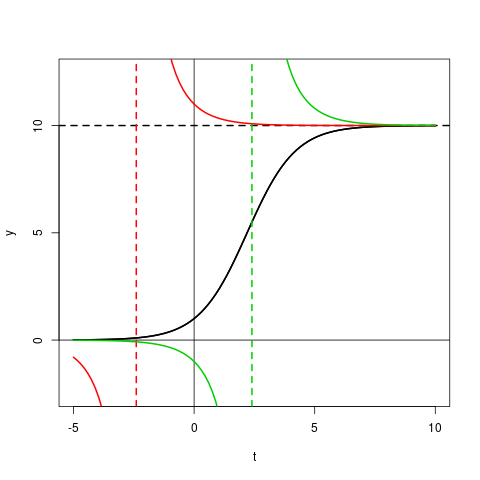
\includegraphics[width=.6\textwidth]{Verhulst-solutions}
  $$
  \item[Stabilité des équilibres :]
  Le point d'équilibre $x^* = K$ est stable pour $y_0 > 0$. Le point d'équilibre $x^* = 0$ est instable.
\end{description}

\remark
Le modèle de Verhulst est un des rares modèles non-linéaires pour lesquels il existe une solution explicite. Il n'est cependant pas nécessaire de disposer d'une solution explicite pour étudier la stabilité d'un équilibre.

\begin{theorem*}[Stabilité ($n = 1$)]
  Pour $n=1$, un point d'équilibre $x^*$ est stable si $F'(x^*) < 0$ et instable si $F'(x^*) > 0$.
\end{theorem*}

\proof Non démontré. \eproof

\remark
On obtient une intuition de ce résultat en étudiant la fonction $h(t) = y(t) - x^*$ au voisinage de $y(t) = x^*$. On a
$$
\dot h(t) = \dot y(t) = F(y(t)) = F(x^* + h(t)) \approx \underset{=0}{\underbrace{F(x^*)}} + F'(x^*) h(t) + o(\|h(t)\|),
$$
$h(t)$ se comporte donc localement comme la solution de 
$$
\dot h(t) = F'(x^*) h(t)
$$
soit $e ^{F'(x^*) t}$ qui tend vers 0 si $F'(x^*) < 0$ et vers l'infini si $F'(x^*) > 0$.

%-------------------------------------------------------------------------------
\paragraph*{Notion de bifurcation.}
De nombreux systèmes dynamiques sont exprimés en fonction de paramètres dont dépendent les points d'équilibre et leur nature. Des valeurs proches des paramètres donnent des points d'équilibres proches et de même nature. La théorie des bifurcations s'intéresse aux régions de l'espace des paramètres au sein desquelles les points d'équilibres restent de même nature : plus précisément elle s'intéresse aux frontières entre ces régions.

%-------------------------------------------------------------------------------
\begin{exercise*}
  Soit le système $\dot y = F(y) = \mu y - y^3$ étudier les points d'équilibre et déterminer leur nature.
\end{exercise*}

\solution{
  On a 
  $$
  F(x) = x(\mu - x^2) = 0 
  \qquad \Leftrightarrow \qquad
  x \in \left\{\begin{array}{ll} 
      \{-\sqrt{\mu}, 0, \sqrt{\mu}\} & \text{si } \mu > 0 \\
      \{0\} & \text{si } \mu \leq 0
    \end{array}\right.
  $$ 
  De plus, 
  $$
  F'(x) = \mu - 3 x^2
  $$
  donc $0$ est toujours instable alors que, pour $\mu > 0$, $-\sqrt{\mu}$ et $\sqrt{\mu}$ sont stables. On peut ainsi tracer le {\em diagramme de bifurcation}.
  $$
  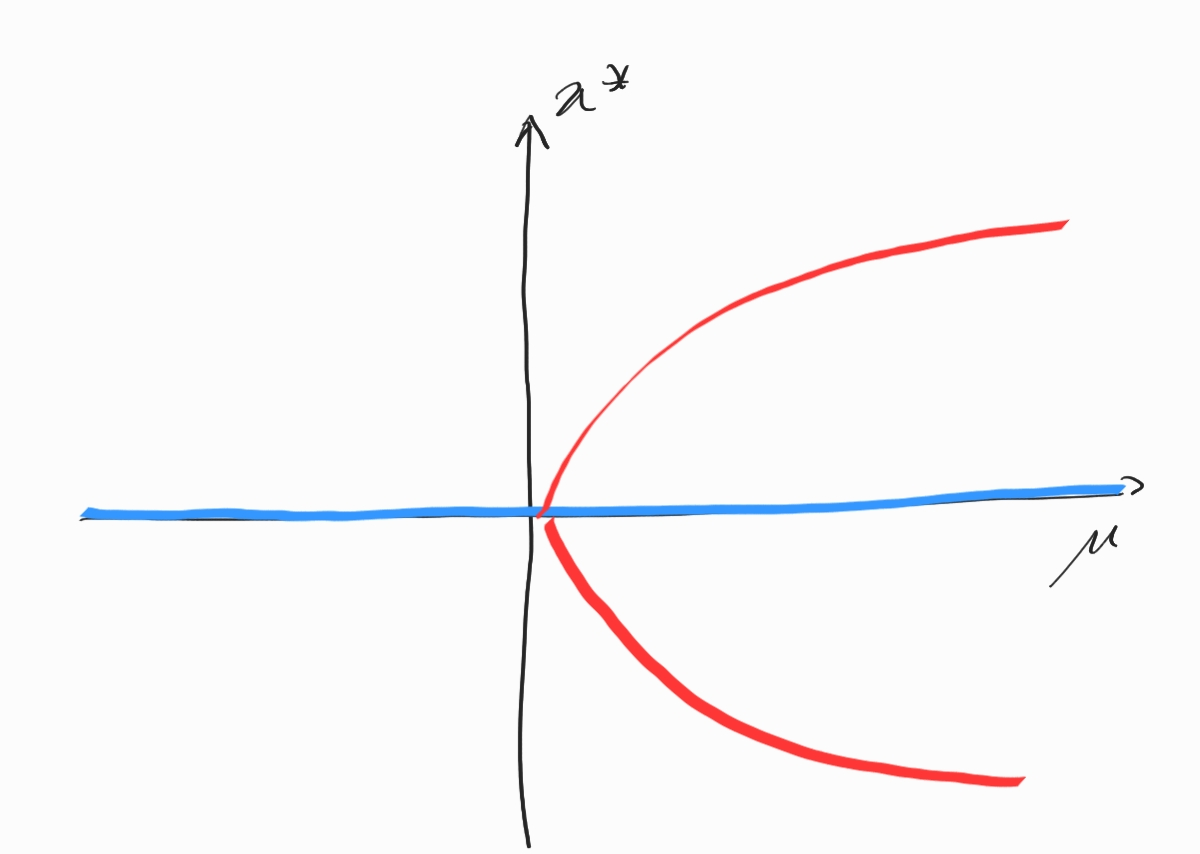
\includegraphics[width=.5\textwidth, trim=0 400 0 0, clip=]{StabiliteSystemeDynamique-Exemple1}
  $$
}

%-------------------------------------------------------------------------------
\textcolor{gray}{
  \begin{exercise*}
    Déterminer les points d'équilibre (et leur nature) du système
    $$
    \dot y = F(y) = \mu y + 2 y^3 - y^5.
    $$
  \end{exercise*}
  %
  \solution{
    On a 
    $$
    F(y) = y(\mu + y^2 - y^4)
    $$
    qui s'annule pour $y = 0$ et pour les solutions de $(\mu + 2 y^2 - y^4)$. En posant, $z = y^2$, $\mu + 2 z - z^2 = 0$ admet des solutions si $\Delta =  4(1 + \mu) \geq 0$, soit $\mu \geq -1$. Ces solutions sont alors $z^* = -1 \pm \sqrt{1+\mu}$. La seule solution possiblement positive est $z^* = -1 + \sqrt{1+\mu}$ et elle l'est ssi $\mu > 1$. \\
    Le système admet donc un unique point fixe $x^*=0$ si $\mu < 1$ et un second point fixe $x^* = -1+\sqrt{1+\mu}$ si $\mu > 1$. \\
    On a de plus
    $$
    F'(x) = \mu + 3 y^2 - 5y^4
    $$
    dont le signe est celui de $\mu$ pour $x=0$ et \todo{nature de $x^* = -1+\sqrt{1+\mu}$ si $\mu > 1$.}
  }}
